\section{编码方法}
\label{sec:lossless-methods}

前两节确定了标准：解码必须唯一，评价看平均码长，下界是熵。Shannon码满足上界，却可能比简单的码还差。本节构造两种实际使用的编码。Huffman编码针对给定的有限符号表，直接求出平均码长最短的前缀码；算术编码不给单个符号分配码字，而是把整条消息对应到$[0,1)$中的一个小区间。两者处理的对象不同，比较时要统一被编码的对象和消息的终止规则。

\subsection{Huffman编码}
\label{sec:lossless-huffman}

在所有二进制前缀码中，哪一个的平均码长最小？前缀码只有有限多种“有用的”码长组合，原则上可以穷举，但符号多时组合数巨大。\term{Huffman编码}（Huffman coding）给出一个只需反复合并的构造\scite{vision-huffman1952}。

\paragraph{主要思想}
从码树的角度看，平均码长是各叶结点深度按概率加权的和。概率小的符号应当放在深处，而最深处的两片叶子一定是兄弟。把这两片叶子合并成它们的父结点，问题就变成一个少一个符号的同类问题。Huffman编码的做法是：每次把概率最小的两个符号合并成一个新符号，新符号的概率是两者之和，直到只剩一个符号；再沿合并的过程从根往下分配$0$和$1$。

要说明这样做是最优的，需要两步：先证明存在一个最优码，其中概率最小的两个符号恰好是最深处的一对兄弟；再证明合并之后的问题与原问题的最优值只相差一个常数。

称前缀码$c^{\star}$为最优的，如果它的平均码长在所有前缀码中最小。最优码存在：任取一个前缀码$c_0$，平均码长不超过$L(c_0)$的前缀码满足
\[
 \ell(x)\leq\frac{L(c_0)}{\min_y p(y)}\quad\text{对每个}x ,
\]
只有有限多种码长组合，其中必有平均码长最小的一个。

\begin{lemma}[最优码的结构]
\label{lem:lossless-optimal-structure}
设$\lvert\mathcal{X}\rvert\geq2$，各$p(x)>0$，$u,v$是概率最小的两个符号（有并列时任取）。则存在最优前缀码$c^{\star}$，使得：
\begin{enumerate}
 \item 若$p(x)>p(y)$，则$\ell(x)\leq\ell(y)$；
 \item $c^{\star}(u)$与$c^{\star}(v)$长度相同且为最大码长，两者只有最后一位不同。
\end{enumerate}
\end{lemma}

\begin{proof}
第一条对每个最优码都成立。若$p(x)>p(y)$而$\ell(x)>\ell(y)$，交换$x,y$的码字，得到的仍是前缀码，平均码长的变化为
\[
 \begin{aligned}
 &p(x)\ell(y)+p(y)\ell(x)-p(x)\ell(x)-p(y)\ell(y)\\
 &\qquad=-\bigl(p(x)-p(y)\bigr)\bigl(\ell(x)-\ell(y)\bigr)<0 ,
 \end{aligned}
\]
与最优性矛盾。

其次，在任一最优码中，设$s$是一个最长的码字，把$s$的最后一位取反得到串$s'$，称为$s$的兄弟。$s'$一定是码字。否则，任何以$s'$开头的码字长度都不小于$\lvert s\rvert$，而$s$已是最长，于是没有码字以$s'$开头；这时删去$s$的最后一位，得到的码仍是前缀码，平均码长减少$p(\cdot)>0$，矛盾。所以最长码字成对出现，每对是兄弟。

最后，取一对最长的兄弟码字，设它们属于符号$y,y'$。把$u$与$y$的码字交换，再把$v$与$y'$的码字交换（若$u$或$v$本来就是$y$或$y'$，相应的交换省去）。由于$p(u)\leq p(y)$而$\ell(u)\leq\ell(y)$（$y$的码长是最大码长），按上面的计算，这一交换使平均码长的变化为
\[
 \bigl(p(y)-p(u)\bigr)\bigl(\ell(u)-\ell(y)\bigr)\leq0 ,
\]
第二次交换同理。交换后的码平均码长不增，仍是最优码，且$u,v$占据最深的一对兄弟。第一条对它仍成立。
\end{proof}

图~\ref{fig:lossless-huffman-exchange}用贯穿例演示交换。码树的深度固定为$1,2,3,3$，若把概率最大的$a$放在深度$3$、概率最小的$d$放在深度$1$，平均码长为$2.5$；交换两者后，平均码长减少
\[
 (0.4-0.1)\times(3-1)=0.6 ,
\]
变为$1.9$。

\begin{BookInlineFigure}
 \centering
 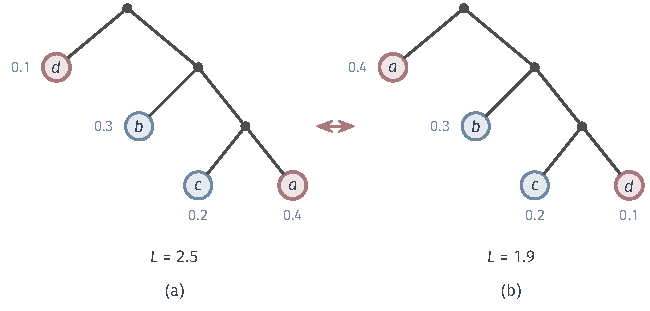
\includegraphics[width=110mm]{figures/07-probability/05-source-coding/tikz/lossless-huffman-exchange/figure.pdf}
 \caption{交换论证。两棵码树形状相同，叶结点旁为概率。(a)把概率$0.4$的$a$放在深度$3$、概率$0.1$的$d$放在深度$1$，平均码长$2.5$。(b)交换两片红色叶子后平均码长降为$1.9$。}
 \label{fig:lossless-huffman-exchange}
\end{BookInlineFigure}

接下来比较合并前后的问题。设$u,v$如引理所述，构造缩减的字母表$\mathcal{X}'$：去掉$u,v$，加入一个新符号$z$，其概率为$p'(z)=p(u)+p(v)$，其余符号概率不变。给定$\mathcal{X}'$上的前缀码$c'$，令
\[
 c(u)=c'(z)0,\qquad c(v)=c'(z)1,\qquad c(x)=c'(x)\ (x\neq u,v),
\]
即把叶子$z$展开成两片兄弟叶子。$c$仍是前缀码，平均码长满足
\begin{equation}
 L(c)=L(c')+p(u)+p(v) ,
 \label{eq:lossless-huffman-reduction}
\end{equation}
因为只有$u,v$的码长比$z$多一位。反过来，若$\mathcal{X}$上的前缀码中$u,v$是兄弟叶子，把它们合并成父结点就得到$\mathcal{X}'$上的前缀码，平均码长的关系同样是式~\eqref{eq:lossless-huffman-reduction}。

\begin{theorem}[Huffman编码的最优性]
\label{thm:lossless-huffman-optimal}
设$\mathcal{X}$有限，$\lvert\mathcal{X}\rvert\geq2$，各$p(x)>0$。Huffman编码的平均码长在所有二进制唯一可译码中最小。
\end{theorem}

\begin{proof}
由Kraft–McMillan不等式，唯一可译码能实现的码长都能由前缀码实现，所以只需与前缀码比较。对符号个数$m=\lvert\mathcal{X}\rvert$作归纳。$m=2$时Huffman编码给出码字$0,1$，平均码长为$1$；唯一可译码不含空码字，平均码长至少为$1$，结论成立。

设结论对$m-1$个符号成立。Huffman编码先合并概率最小的$u,v$，在缩减字母表$\mathcal{X}'$上得到Huffman码$h'$，再把$z$展开，得到$\mathcal{X}$上的码$h$。由式~\eqref{eq:lossless-huffman-reduction}，
\[
 L(h)=L(h')+p(u)+p(v).
\]
取引理~\ref{lem:lossless-optimal-structure}给出的最优码$c^{\star}$，其中$u,v$是兄弟叶子，合并得到$\mathcal{X}'$上的前缀码$c'$，同样有
\[
 L(c^{\star})=L(c')+p(u)+p(v).
\]
由归纳假设，$h'$在$\mathcal{X}'$上最优，$L(h')\leq L(c')$。两式相减得$L(h)\leq L(c^{\star})$，所以$h$也是最优码。
\end{proof}

式~\eqref{eq:lossless-huffman-reduction}还给出一个算平均码长的捷径：每合并一次，平均码长增加被合并两项的概率之和。所以Huffman码的平均码长等于各次合并所得新结点的概率之和。

\paragraph{计算过程}
下面在贯穿例$p=(0.4,0.3,0.2,0.1)$上逐步执行。

\needspace{6\baselineskip}
\paragraph{变量}
\begin{itemize}
 \item 待合并结点的集合$\mathcal{Q}$：每个结点是一棵子树，带有权重，即子树中所有叶结点的概率之和。实现时用按权重排序的优先队列。
 \item 子树内部的连接：每个内部结点记住它的两个子结点，以及分别通向它们的边上的位$0$或$1$。
 \item 并列规则：权重相同时，先进入$\mathcal{Q}$的结点先取出。原始符号在初始化时进入，合并产生的结点后进入。
\end{itemize}

\paragraph{初始化}
每个符号是一个只有一片叶子的子树，权重为它的概率，全部放入$\mathcal{Q}$。例中
\[
 \mathcal{Q}=\{a:0.4,\ b:0.3,\ c:0.2,\ d:0.1\}.
\]

\needspace{6\baselineskip}
\paragraph{每轮更新}
当$\mathcal{Q}$中多于一个结点时：
\begin{enumerate}
 \item \textbf{取出两个最小权重。}从$\mathcal{Q}$中依次取出权重最小的结点$s_1$与次小的结点$s_2$。例中第一轮取出$d$（$0.1$）与$c$（$0.2$）。
 \item \textbf{合并。}新建内部结点$t$，以$s_1,s_2$为子结点，通向$s_1$的边记$0$，通向$s_2$的边记$1$，权重为两者之和。例中第一轮
 \[
  t_1=\{d,c\},\qquad 0.1+0.2=0.3 .
 \]
 \item \textbf{放回。}把$t$放入$\mathcal{Q}$。例中第一轮后
 \[
  \mathcal{Q}=\{a:0.4,\ b:0.3,\ t_1:0.3\}.
 \]
\end{enumerate}
例中第二轮，$b$与$t_1$的权重都是$0.3$，按并列规则先取出$b$，再取出$t_1$，合并为权重$0.6$的结点$t_2$，$b$一侧记$0$，$t_1$一侧记$1$：
\[
 \mathcal{Q}=\{a:0.4,\ t_2:0.6\}.
\]
第三轮取出$a$与$t_2$，合并为权重$1$的根结点$t_3$，$a$一侧记$0$，$t_2$一侧记$1$，$\mathcal{Q}$中只剩一个结点，合并结束。图~\ref{fig:lossless-huffman-steps}画出各轮之后的森林。

\begin{BookInlineFigure}
 \centering
 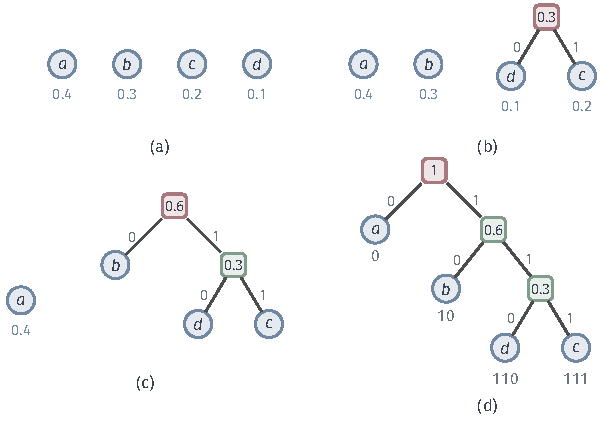
\includegraphics[width=102mm]{figures/07-probability/05-source-coding/tikz/lossless-huffman-steps/figure.pdf}
 \caption{贯穿例的Huffman合并。蓝圈为原始符号及其概率，方框为合并产生的结点及其权重，红框是该轮新产生的结点，边旁为分配的位。(a)初始；(b)合并$d,c$；(c)合并$b$与$\{d,c\}$；(d)合并$a$得到根，叶结点下方为码字。}
 \label{fig:lossless-huffman-steps}
\end{BookInlineFigure}

\paragraph{读出码字}
从根出发走到每片叶子，依次写下经过的位，就是该符号的码字。例中
\[
 a\mapsto0,\qquad b\mapsto10,\qquad d\mapsto110,\qquad c\mapsto111 .
\]
码长为$1,2,3,3$。按合并新结点的权重求和，
\[
 L=0.3+0.6+1.0=1.9 ,
\]
与按定义逐项计算一致。最终得到的码长与第~\ref{sec:lossless-model}节的码表相同，只是$c,d$的码字互换；两者长度相同，平均码长都是$1.9$，冗余为$1.9-1.846=0.054$。由定理~\ref{thm:lossless-huffman-optimal}，在这个概率表下没有平均码长小于$1.9$的唯一可译码。

\paragraph{算法分析}
用二叉堆实现优先队列时，每轮取出两次、放入一次，各需$O(\log m)$次比较，共$m-1$轮，总计算量为$O(m\log m)$；若概率已经排好序，可以用两个先进先出队列在$O(m)$时间内完成。并列规则不同时，得到的码树和码长都可能不同，但由定理~\ref{thm:lossless-huffman-optimal}，平均码长相同。最长码字可以长达$m-1$位，例如概率按$1/2,1/4,1/8,\dots$递减时码树退化成一条链。

最优性的范围要说清楚。定理只断言：对一个给定的有限字母表和给定的概率表，在逐符号的二进制唯一可译码中，Huffman码平均码长最短。它不说明每个符号至少要花这么多位；若把若干符号合成一块再编码，被编码的字母表就换成了$\mathcal{X}^n$，有$\lvert\mathcal{X}\rvert^n$个“符号”，Huffman码要对这个大字母表重新构造，平均到每个原始符号上可以更短（第~\ref{sec:lossless-block-limits}节）。代价是码表规模随块长指数增长。

\subsection{算术编码}
\label{sec:lossless-arithmetic}

Huffman码给每个符号整数位，概率极不均匀时，一个符号可能只含零点几位信息，却至少要花一位。另一条路是不给符号分配码字，而给整条消息分配码字。\term{算术编码}（arithmetic coding）用一个逐步缩小的区间来做这件事\scite{math-witten1987arithmetic}。

\paragraph{主要思想}
把$[0,1)$看成单位质量，按概率分给各个符号：贯穿例中$a$占$[0,0.4)$，$b$占$[0.4,0.7)$，$c$占$[0.7,0.9)$，$d$占$[0.9,1)$。读到第一个符号，就留下它的那一段；在这一段里再按同样的比例分给四个符号，读到第二个符号再留下相应的一小段；如此继续。读完整条消息时剩下的区间，长度恰好是这条消息的概率。

用公式写出来。给$\mathcal{X}$中的符号排定顺序，记累积概率
\[
 F(x)=\sum_{y\prec x}p(y),
\]
其中$y\prec x$表示$y$排在$x$之前。贯穿例按$a,b,c,d$排序，$F(a)=0$，$F(b)=0.4$，$F(c)=0.7$，$F(d)=0.9$。消息$x_{1:n}$对应的区间$[\mathrm{lo}_k,\mathrm{lo}_k+w_k)$按下式逐步更新：
\begin{equation}
 \mathrm{lo}_0=0,\quad w_0=1;\qquad
 \mathrm{lo}_k=\mathrm{lo}_{k-1}+w_{k-1}F(x_k),\quad w_k=w_{k-1}\,p(x_k).
 \label{eq:lossless-arith-update}
\end{equation}
第$k$步把当前区间按比例切开，留下第$k$个符号的那一份。由此$w_n=\prod_{k}p(x_k)$，按式~\eqref{eq:lossless-product}正是$p(x_{1:n})$。记$J(x_{1:n})=[\mathrm{lo}_n,\mathrm{lo}_n+w_n)$。

固定消息长度$n$，所有长度为$n$的消息的区间$J(x_{1:n})$两两不交，并且铺满$[0,1)$。对$n$归纳：$n=0$时只有$[0,1)$；长度为$k$的消息的区间由长度为$k-1$的前缀的区间按概率切成$\lvert\mathcal{X}\rvert$份得到，各份不交且铺满原区间。

剩下的问题是怎样用尽量少的位说出“消息的区间是哪一个”。办法与Kraft不等式的证明相同：找一个完全落在$J(x_{1:n})$内的二进区间，发送它对应的二进制串。取
\begin{equation}
 \ell=\Bigl\lceil\log_2\frac{1}{w_n}\Bigr\rceil+1,\qquad
 k=\bigl\lceil\mathrm{lo}_n2^{\ell}\bigr\rceil ,
 \label{eq:lossless-arith-codeword}
\end{equation}
码字是整数$k$的$\ell$位二进制表示（不足$\ell$位时前面补$0$），它对应二进区间$[k2^{-\ell},(k+1)2^{-\ell})$。

这个二进区间落在$J(x_{1:n})$内。左端：$k\geq\mathrm{lo}_n2^{\ell}$，所以$k2^{-\ell}\geq\mathrm{lo}_n$。右端：$k<\mathrm{lo}_n2^{\ell}+1$，再由$\ell$的取法$2^{-\ell}\leq w_n/2$，于是
\[
 (k+1)2^{-\ell}<\mathrm{lo}_n+2\cdot2^{-\ell}\leq\mathrm{lo}_n+w_n .
\]
同一长度的不同消息区间不交，它们的二进区间也不交，所以这些码字中没有一个是另一个的前缀：对固定的$n$，算术编码是$\mathcal{X}^n$上的前缀码。码长满足
\begin{equation}
 \ell<\log_2\frac{1}{p(x_{1:n})}+2 ,
 \label{eq:lossless-arith-length}
\end{equation}
对消息取期望，平均码长小于$nH(X)+2$，每符号小于$H(X)+2/n$。消息越长，这额外的两位摊得越薄。

解码是同一过程的逆向。设收到码字，算出$v=k2^{-\ell}$，它落在$J(x_{1:n})$中。第一个符号是唯一满足$F(x)\leq v<F(x)+p(x)$的$x$；把$v$换成$(v-F(x_1))/p(x_1)$，即在留下的子区间中重新标定到$[0,1)$，再按同样的规则读出第二个符号，如此重复$n$次。解码器必须使用与编码器完全相同的符号顺序和概率。

\paragraph{计算过程}
下面用贯穿例对消息$abac$逐步演示，$n=4$事先约定。

\needspace{6\baselineskip}
\paragraph{变量}
\begin{itemize}
 \item 概率表$p(x)$与累积概率表$F(x)$：各$\lvert\mathcal{X}\rvert$个数，编码器与解码器共享。
 \item $\mathrm{lo}$：当前区间的左端点。
 \item $w$：当前区间的长度。
 \item 消息长度$n$：事先约定，或按下文的终止规则处理。
\end{itemize}

\paragraph{初始化}
$\mathrm{lo}=0$，$w=1$。例中$F=(0,0.4,0.7,0.9)$，$p=(0.4,0.3,0.2,0.1)$。

\needspace{6\baselineskip}
\paragraph{每轮更新}
对$k=1,\dots,n$，读入符号$x_k$：
\begin{enumerate}
 \item \textbf{移左端。}按式~\eqref{eq:lossless-arith-update}，$\mathrm{lo}\leftarrow\mathrm{lo}+w\,F(x_k)$。
 \item \textbf{缩长度。}$w\leftarrow w\,p(x_k)$。
\end{enumerate}
例中四轮的结果如下（先算左端，再用旧的$w$乘概率）：
\[
 \begin{aligned}
 &a:&\mathrm{lo}&=0+1\times0=0, & w&=1\times0.4=0.4,\\
 &b:&\mathrm{lo}&=0+0.4\times0.4=0.16, & w&=0.4\times0.3=0.12,\\
 &a:&\mathrm{lo}&=0.16+0.12\times0=0.16, & w&=0.12\times0.4=0.048,\\
 &c:&\mathrm{lo}&=0.16+0.048\times0.7=0.1936, & w&=0.048\times0.2=0.0096.
 \end{aligned}
\]
读完$n$个符号后结束，最终区间为
\[
 J(abac)=[0.1936,\,0.2032),\qquad w_4=0.0096=p(abac).
\]

\paragraph{输出码字}
由式~\eqref{eq:lossless-arith-codeword}，
\[
 \ell=\lceil6.703\rceil+1=8,\qquad k=\lceil0.1936\times256\rceil=\lceil49.56\rceil=50 ,
\]
码字是$50$的$8$位二进制表示$00110010$，对应二进区间
\[
 [50/256,\,51/256)=[0.1953,\,0.1992)\subset[0.1936,\,0.2032).
\]
图~\ref{fig:lossless-arith-intervals}逐行画出区间的缩小过程。这条消息的自信息是$\log_2(1/0.0096)=6.703$位，算术编码用了$8$位，比上一小节的Huffman码字串$0\,10\,0\,111$多一位。对这样短的消息，式~\eqref{eq:lossless-arith-length}中的两位额外开销相当可观；它的好处要在长消息中才显现。

\begin{BookInlineFigure}
 \centering
 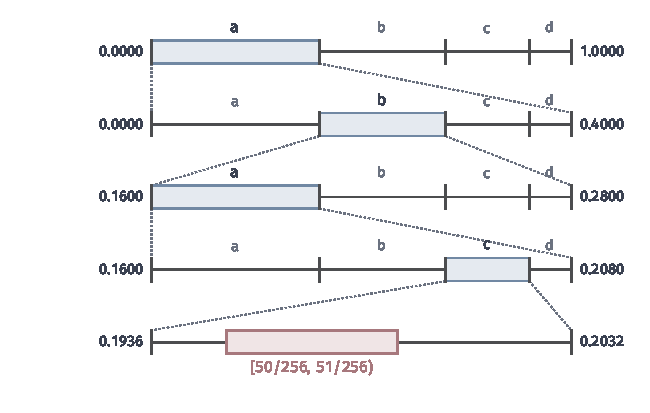
\includegraphics[width=110mm]{figures/07-probability/05-source-coding/matplotlib/lossless-arith-intervals/figure.pdf}
 \caption{算术编码消息$abac$。每一行把当前区间放大到同样宽度，两侧数字为区间端点，按$4:3:2:1$切给$a,b,c,d$；浅蓝格是读到的符号留下的子区间，虚线把它放大到下一行。最后一行是最终区间$[0.1936,0.2032)$，红框是码字$00110010$对应的二进区间。}
 \label{fig:lossless-arith-intervals}
\end{BookInlineFigure}

同样长度的另一条消息$abad$只在最后一步不同：$\mathrm{lo}=0.16+0.048\times0.9=0.2032$，$w=0.0048$，于是$\ell=\lceil7.703\rceil+1=9$，$k=\lceil0.2032\times512\rceil=105$，码字为$001101001$。它与$00110010$在第$6$位就不同，谁也不是谁的前缀，这正是两条消息的区间$[0.1936,0.2032)$与$[0.2032,0.2080)$不交的结果。

\paragraph{解码}
解码器收到$00110010$，得$v=50/256=0.1953$，逐步读出：
\[
 \begin{aligned}
 &v=0.1953\in[0,0.4) &&\Rightarrow a, & v&\leftarrow0.1953/0.4=0.4883,\\
 &v=0.4883\in[0.4,0.7) &&\Rightarrow b, & v&\leftarrow(0.4883-0.4)/0.3=0.2943,\\
 &v=0.2943\in[0,0.4) &&\Rightarrow a, & v&\leftarrow0.2943/0.4=0.7357,\\
 &v=0.7357\in[0.7,0.9) &&\Rightarrow c .
 \end{aligned}
\]
读满$n=4$个符号后停止，恢复出$abac$。

\paragraph{终止规则}
上面的码对固定的$n$是前缀码，不同长度的消息之间却可能冲突：同一个码字所在的二进区间，既落在某条长度为$4$的消息的区间里，也落在它的前缀$aba$的区间里。所以接收方必须知道消息在哪里结束。常用两种约定。一是事先约定或单独传送长度$n$；单独传送时，用一个整数的前缀码，大约需要$2\log_2n$位。二是在字母表中加入终止符号，给它一个小概率$\varepsilon$，其余符号的概率乘以$1-\varepsilon$；消息总以终止符号结束，于是“消息加终止符”组成的集合中没有一条是另一条的前缀。终止符号的代价是消息末尾多出$\log_2(1/\varepsilon)$位，每个普通符号多出$\log_2(1/(1-\varepsilon))$位。

\paragraph{有限精度}
上面的计算用的是精确实数，消息长时$w$小到无法用浮点数表示。实际实现用整数：概率表写成整数频数$f(x)$，总和为$T$；区间端点用$B$位整数表示。每读一个符号，按频数比例切分整数区间并向下取整。每当区间整个落在$[0,1/2)$或$[1/2,1)$中，最高位已经确定，立即输出这一位，并把区间放大一倍，使区间长度保持在一个固定范围内；区间跨越中点但很窄时，记下“待定位”的个数，等以后确定方向再一并输出。

整数实现能正确解码的关键，是编码器与解码器做完全相同的整数运算和取整：只要两边一致，取整只是把每个子区间的长度稍微改动，改动后的子区间仍两两不交、铺满当前区间。取整的代价是码长比式~\eqref{eq:lossless-arith-length}稍长，$B$足够大时这个损失很小。此外每个可能出现的符号都需要$f(x)\geq1$，否则它的子区间长度为零，无法编码。

\paragraph{模型与实际概率}
编码器和解码器用的概率表$q$称为模型，它可以与信源的真实分布$p$不同。只要两边用同一个$q$，并且消息中出现的每个符号都有$q(x)>0$，上面的论证不变，只需把$p$换成$q$：码长满足
\[
 \ell<\log_2\frac{1}{q(x_{1:n})}+2 ,
\]
解码仍然正确。模型不准只让码长变长，对独立同分布消息，平均每符号码长约为$H(X)+D_{\mathrm{KL}}(p\Vert q)$，第~\ref{sec:lossless-finite-resources}节将给出这一点的精确界。

若模型给一个实际出现的符号零概率，$q(x_k)=0$，则$w$在这一步变成$0$，区间消失，这条消息无法编码。这不是“码长变长”的问题，而是编码本身无法继续。所以模型必须给每个可能出现的符号留下正概率。

模型也可以随已读的符号改变，只要编码器和解码器按同一规则更新：把式~\eqref{eq:lossless-arith-update}中的$p(x_k)$与$F(x_k)$换成依赖于$x_{1:k-1}$的条件概率与累积概率，区间长度就变成这些条件概率的乘积，上面的论证照样成立。这使算术编码可以配合任意按顺序给出概率的模型，而Huffman码要求事先给定一个固定的概率表。

\paragraph{与Huffman编码比较}
比较两种方法时，必须让它们编码同一个对象，按同一个终止规则。Huffman码是逐符号的前缀码，消息结束靠约定长度或额外的码字；按长度为$n$的整条消息计算，它的平均码长为$n\times1.9$，每符号$1.9$位。算术编码在$n$已知时，每符号平均码长小于
\[
 H(X)+\frac{2}{n}=1.846+\frac{2}{n} ,
\]
$n=4$时这个上界是$2.346$，比Huffman码差；$n=40$时为$1.896$，已低于Huffman码。

图~\ref{fig:lossless-arith-length}在一条长$400$的随机消息上验证这些数值。用真实模型$p$编码时，每符号码长从短消息时的约$3$位逐步降到$1.855$位，接近熵$1.846$；用均匀模型$q(x)=1/4$编码时，码长恰为$2n+1$，每符号趋于$2$，即$H+D_{\mathrm{KL}}(p\Vert q)=1.846+0.154$。右图显示，在每个前缀长度上，码长与自信息之差都落在$[1,2)$中，这正是式~\eqref{eq:lossless-arith-codeword}的取整与$+1$造成的。

\begin{BookInlineFigure}
 \centering
 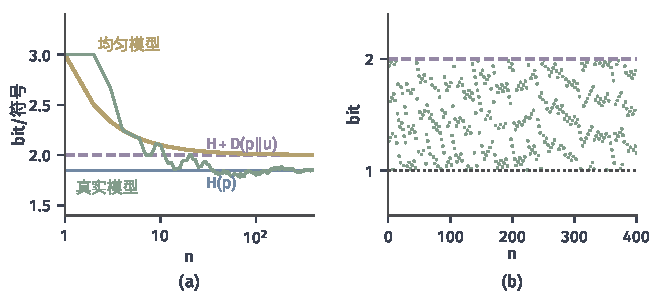
\includegraphics[width=110mm]{figures/07-probability/05-source-coding/matplotlib/lossless-arith-length/figure.pdf}
 \caption{一条由贯穿例信源独立生成、长$400$的消息（随机种子$7$）。(a)各前缀长度$n$下算术编码的每符号码长，横轴为对数坐标：绿线用真实模型，黄线用均匀模型；蓝线为熵$H=1.846$，紫色虚线为$H+D_{\mathrm{KL}}(p\Vert u)=2$。(b)真实模型下码长与消息自信息之差，所有点落在$[1,2)$中。}
 \label{fig:lossless-arith-length}
\end{BookInlineFigure}
